\documentclass[12pt,twoside]{report}
% includes
\usepackage{csquotes}
\usepackage{titlesec}
\usepackage{geometry}         % page size
\usepackage[utf8]{inputenc}     % encoding
\usepackage{palatino}           % font
\usepackage[english]{babel}    % language
\usepackage{graphicx}           % images
\usepackage{indentfirst}        % indentation
\usepackage[nottoc]{tocbibind}  % table of contents style
\usepackage[unicode]{hyperref}  % references from the table of contents
\usepackage[sorting=none]{biblatex}
\usepackage{array}
\newcolumntype{P}[1]{>{\centering\arraybackslash}p{#1}}
\addbibresource{mybib.bib}
% includes options
\geometry{  a4paper,            % scientific thesis standard
            left=3cm,
            right=2cm,
            top=1.5cm,
            bottom=3cm,
 }
\graphicspath{{images/}}        % path where the images are located
\setlength{\parindent}{1cm}     % paragraph indentation

% other options
\linespread{1.5}                % space between lines
\renewcommand*\contentsname{Cuprins}    % table of contents name
\newcommand{\cchapter}[1]{\chapter[#1]{\centering #1}}
% the document content
\usepackage{titlesec}
\titleformat{\chapter}[display]
  {\filleft\Huge}
  {\chaptername\ \thechapter}
  {3ex}
  {\bfseries}
\titlespacing*{\chapter}
  {0pt}
  {-15pt}
  {60pt}
  
\begin{document}
    % macros (global)
    \newcommand{\university}    {National Institute of Technology Silchar}
\newcommand{\universityg}   {National Institute of Technology Silchar} % genitive
\newcommand{\faculty}       {Department of Computer Science \& Engineering}
\newcommand{\facultyg}      {Department of Computer Science \& Engineering} % genitive
\newcommand{\speciality}    {Software Defined Networks}
\newcommand{\promotion}     {May, 2020}                                  %<---------

\newcommand{\thesistype}    {M.Tech Thesis}
\newcommand{\thesistitle}   {System Utilization Analysis of \\\vspace{-5mm}SDN/OpenFlow Controllers: Ryu Versus Pox}    %<---------

\newcommand{\authorlast}    {Jee}                               %<---------
\newcommand{\authorfirst}   {Gautam}
\newcommand{\authornamefl}  {\authorfirst \space \authorlast} % first name first
\newcommand{\authornamelf}  {\authorlast \space \authorfirst} % last name first
\newcommand{\authorbirth}   {06 May 1996}                      %<---------
\newcommand{\authoraddress} {NIT Silchar} %<---------
\newcommand{\authorcnp}     {(18-2-5-107)}                         %<---------

\newcommand{\session}       {2018-2020}                       %<---------
\newcommand{\coordinator}   { Umakanta Majhi\\ \Large (Assistant Professor)}               %<---------

\newcommand{\dottedline}    {............................}
    % front-matter
    \pagenumbering{gobble}
    % define the cover page
\begin{titlepage}
    \begin{center}
    
        % thesis title
        \vspace{4cm}
        \LARGE
        \textbf{\thesistitle}
        
        % author
        \vspace{2.5cm}
        \large{A Thesis Submitted in\\
Partial Fulfillment of the Requirements for the\\
Degree of Master of Technology}\\[8pt]
        % the faculty logo
        \vspace{2.5cm}
        
\includegraphics[width=0.3\textwidth]{images/NIT_Silchar_logo.png}\\
        \vspace{2cm}
        \LARGE
        \textbf{\authornamefl}\\
        \authorcnp\\
        \vspace{2.5cm}
        % the university
        \Large
        {\textbf{\faculty}}\\
        \large
        \MakeUppercase{\university}\\
        \Large \promotion
        
    \end{center}
\end{titlepage}
    % define the title page
\begin{titlepage}
    \begin{center}
        % thesis title
        \vspace{1cm}
        \LARGE
        \textbf{\thesistitle}
        
        % author
        \vspace{1cm}
        \large{A Thesis Submitted in\\
Partial Fulfillment of the Requirements for the\\
Degree of Master of Technology}\\[8pt]
        
        % the faculty logo
        \vspace{1cm}
        
\includegraphics[width=0.3\textwidth]{images/NIT_Silchar_logo.png}\\
        \vspace{0.5cm}
        \LARGE
        \textbf{\authornamefl}\\
        \authorcnp\\
        \vspace{1.5cm}
        % scientific coordinator
        \Large
        under the supervision of\\
        \LARGE
        \textbf{\coordinator}\\
        \vspace{1.5cm}
        % the university
        \Large
        \textbf{\faculty}\\
        \Large
        {\university}\\
        \Large \promotion
    \end{center}
\end{titlepage}
    % \addcontentsline{toc}{chapter}{Recommendation}
\vspace*{0.5\fill}
\setlength{\headsep}{0.4in}
\rule{\linewidth}{1mm}
\begin{minipage}{0.2\textwidth}

\includegraphics[width=3cm,keepaspectratio]{images/NIT_Silchar_logo.png}
\end{minipage}
\begin{minipage}{\textwidth}
\large{Department of Computer Science \& Engineering}\\
\large{\MakeUppercase{NATIONAL INSTITUTE OF TECHNOLOGY SILCHAR}}
\end{minipage}

{\noindent\rule{\linewidth}{1mm}} \vspace{0.25in}

\begin{center}

{\bf \LARGE RECOMMENDATION SHEET}

\end{center}


Submission Type (for Evaluation/Record): \textbf{Record} \linebreak
Title of the Thesis: \textbf{System Utilization Analysis of SDN/OpenFlow Controllers: Ryu Versus Pox}
\vspace{0.25in} \linebreak
Degree(PhD,M.Tech./M.Sc./MBA): \textbf{Master of Technology} \linebreak
Name of Student: \textbf{Gautam Jee} \linebreak
Registration Number: \textbf{18-2-5-107} \linebreak
Name of Department: \textbf{Department of Computer Science & Engineering} \linebreak
Name(s) of Supervisor(s): \textbf{Umakanta Majhi} \linebreak
\begin{flushright}
(Signature of the Student)
\end{flushright}
\vspace{0.5cm}
\underline{Recommendation of the Examiners} \linebreak
Above thesis is recommended for submission.
\textbf{Prof. Nidul Sinha}(External Expert)
\textbf{Dr. U. Chakraborty}(Expert from allied Department):
\textbf{Mr. P.K. Nath}(Expert from CSE Department):
\textbf{Dr. Arup Bhattacharjee}(Chairperson):
\textbf{Umakanta Majhi} (Supervisor)
\begin{minipage}{0.5\textwidth}
\begin{flushleft}
For Academic/Department office use \linebreak
Thesis received on:
Signature of the Dealing Assistant/AR:
\end{flushleft}
\end{minipage}
\begin{minipage}{0.4\textwidth}
\vspace*{\fill}
\end{minipage}
\pagebreak
    \clearpage
    \setcounter{page}{1}
    \pagenumbering{roman}
    \addcontentsline{toc}{chapter}{Declaration}
\vspace*{0.5\fill}
\setlength{\headsep}{0.4in}
\noindent \rule{\linewidth}{1mm}
\begin{minipage}{0.2\textwidth}

\includegraphics[width=3cm,keepaspectratio]{images/NIT_Silchar_logo.png}
\end{minipage}
\begin{minipage}{\textwidth}
\large{Department of Computer Science \& Engineering}\\
\large{\MakeUppercase{NATIONAL INSTITUTE OF TECHNOLOGY SILCHAR}}
\end{minipage}

{\noindent\rule{\linewidth}{1mm}} \vspace{0.25in}

\begin{center}

{\bf \LARGE Declaration}

\end{center}

\par

Thesis Title: \textbf{System Utilization Analysis of SDN/OpenFlow Controllers: Ryu Versus Pox}

\vspace{0.25in}

Degree for which the Thesis is submitted: \textbf{Master of Technology}

\vspace{0.25in}

I declare that the presented thesis represents largely my own ideas and work in my own
words. Where others ideas or words have been included, I have adequately cited and listed
in the reference materials. The thesis has been prepared without resorting to plagiarism. I
have adhered to all principles of academic honesty and integrity. No falsified or fabricated
data have been presented in the thesis. I understand that any violation of the above will
cause for disciplinary action by the Institute, including revoking the conferred degree, if
conferred, and can also evoke penal action from the sources which have not been properly
cited or from whom proper permission has not been taken.


\vspace{0.5cm}
\begin{minipage}{0.5\textwidth}
\begin{flushleft}
Date :
\end{flushleft}
\end{minipage}
\begin{minipage}{0.4\textwidth}
\begin{flushright}

\vspace{0.5cm}

\vspace{0.25in}

\textbf{Gautam Jee}

Reg. No- 18-2-5-107
\end{flushright}
\vspace*{\fill}
\end{minipage}
\pagebreak


    \addcontentsline{toc}{chapter}{Certificate}
\vspace*{0.5\fill}
\setlength{\headsep}{0.4in}
\noindent \rule{\linewidth}{1mm}
\begin{minipage}{0.2\textwidth}

\includegraphics[width=3cm,keepaspectratio]{images/NIT_Silchar_logo.png}
\end{minipage}
\begin{minipage}{\textwidth}
\large{Department of Computer Science \& Engineering}\\
\large{\MakeUppercase{NATIONAL INSTITUTE OF TECHNOLOGY SILCHAR}}
\end{minipage}

{\noindent \rule{\linewidth}{1mm}} \vspace{0.25in}



\begin{center}



{\bf \LARGE Certificate}

\end{center}

\par
It is certified that the work contained within this thesis entitled \textbf{``System \linebreak Utilization Analysis of SDN/OpenFlow Controllers: Ryu Versus Pox''} submitted by \linebreak GAUTAM JEE Scholar no: 18-2-5-107 for the award of M.Tech is absolutely based on his own work carried out under my supervision and this thesis has not been submitted elsewhere for any degree.
\vspace{1cm}

\begin{minipage}{0.3\textwidth}
\begin{flushleft}
\vspace{1in}
Date  : \\
\vspace{0.3cm}
Place : 
\end{flushleft}
\end{minipage}
\begin{minipage}{0.65\textwidth}
\begin{flushright}
\vspace{5cm}
\textbf{Umakanta Majhi}\\
\textbf{Assistant Professor}
 
\textbf{Department of Computer Science \& Engineering}

\textbf{NIT Silchar, India }                                        \end{flushright}
\end{minipage}
\pagebreak

    \addcontentsline{toc}{chapter}{Abstract}
\setlength{\headsep}{0.4in}
\vspace*{5cm}
\begin{center}

{\bf \LARGE Abstract}

\end{center}

{\noindent \rule{\linewidth}{1mm}} \vspace{0.25in}

\par
Over the years, a number of Software Defined Network (SDN) operating systems have been developed in different languages architectures. The tier of importance in an SDN architecture is its control plane which is governed by the entity called ``Controller''. Hence there is a need to understand the merits and demerits of these controllers so that one may choose an appropriate implementation for a network scenario. Here, a study of two SDN controllers is performed with the aim to understand the system utilization of SDN Controller under heavy traffic and gives a better idea about its running nature, system, bottlenecks, etc. which could further let the developers know the improvement areas to work in its upcoming versions.
\vspace*{\fill}
\pagebreak
    \addcontentsline{toc}{chapter}{Acknowledgement}
\setlength{\headsep}{0.4in}
\vspace*{5cm}
\begin{center}

{\bf \LARGE Acknowledgement}

\end{center}

{\noindent \rule{\linewidth}{1mm}} \vspace{0.25in}

\par
Achievements in life are always obtained through some key ingredients added into the recipe which is your work. A spoon of guidance, a touch of inspiration, a squeeze of determination and heaps of blessings are the most crucial among them. This work would not have been possible without the constant support and motivation given to me by my teachers and family.

Hence, I take this opportunity to express gratitude to my guide and mentor, \textbf{Umakanta Majhi}, Assistant Professor, Department of Computer Science and Engineering, National Institute of Technology, Silchar for his expert guidance, innovative suggestions, constant encouragement and patience with which he handled me and the project.His calm minded approach to the project instilled the confidence within me and taught me to embrace the challenges that were ahead.

I am forever grateful to \textbf{Dr. Samir Kumar Borgohain}, Head of the Department, Department of Computer Science and Engineering for his encouragement and considerations throughout my research work. His constant support has been invaluable to me in the pursuit of my research work.

Finally, I express my gratitude to my beloved parents, family and friends who directly or indirectly extended help and prayers to make this thesis successful. 


\vspace{1.5cm}

\begin{flushright}

\textbf{Gautam Jee}

Reg. No- 18-2-5-107
\end{flushright}
\pagebreak

    % table of contents
    \protect\cleardoublepage
    \tableofcontents
    \listoffigures
    \listoftables
    % chapters
    \clearpage
    \setcounter{page}{1}
    \pagenumbering{arabic}
    \chapter{Introduction}

The term network system passes on, an association of various PCs. For the most part, these systems have two kinds of availability, which are wired and remote. As on account of any innovation, it is development came out as a need. For any country, its most extreme need is to keep up military certainty. During the change from the electrical and mechanical age to the electronic age, everything from regular family unit things to bank the board experienced a significant overhaul. Normally, this implied the safeguarded area grasped innovation sometime before. The entire first network system was essential and was set up in a military resistance venture called ARPANET, representing the Advanced Research Projects Agency Network. It was the beginning stage of the current web. PC arranges throughout the years have developed a wide margin regarding highlights, intricacy, and power. That as well as it has extended its scope to the business and new parts. In these advanced occasions, terms such as switches and passages, are recognizable to even the layman.
\vspace{5mm}
\section{Traditional Networks}

Even something as new and intense as network systems have demonstrated age. The maturing of innovation is by all accounts a lot snappier than people. Inside two decades, it built up an area of systems classified as traditional networks. Traditional networks are the spearheading plan of networks. Adam Smith of computer networking had a structure that was solid for the time and had no issues for quite a while. Indeed, even today, the traditional network system engineering cannot be blamed as is yet a subject of innovative work. Nevertheless, concerning each innovation that exists, there will be advantages and disadvantages.

\begin{figure}[!hbt]
    \centering
    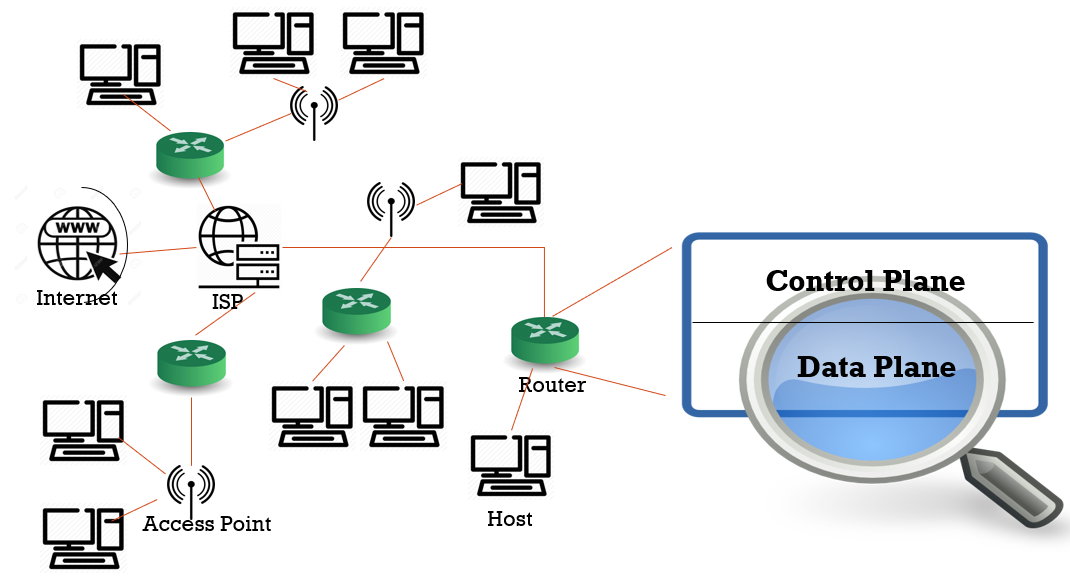
\includegraphics[width=\textwidth,keepaspectratio]{images/TRADITIONAL-NETWORK.png}
    \caption{Traditional Networks \cite{sdnimages}}
    \label{fig:Tradnets}
\end{figure}

   The computer network was developed for the sole purpose of communication. So this meant carrying digital information from one machine to another remote machine, via wire or air. It is similar to the case of sending a post from one individual to another. A post was given to the post office, which redirects it to another post office, which would be closest to the receiver's address.
    
    This task of forwarding the post is the same in the case of computer networks and termed as routing. In computer networks, no humans are interfering; rather, there are individual devices in charge of performing this data forwarding. The task of routing is delegated to devices called routers, which make up a fair share of the entire global network today.
    
    Routers play the most crucial role in today's network, i.e., forwarding packets via specific routes by figuring out the current situation of the neighboring network devices and keeping track of the connected devices. Similar to how everybody has a PO box attached to their address, every device in a local network is registered under a router. These routers are scattered throughout the network and are necessarily the backbone of the network. The same reason is why this technique has been researched for years so that it has good fault tolerance and error correction. Such a network where there are millions of packet forwarding devices ensures redundancy, and as there is no single point of vulnerability.
    \vspace{2mm}
    
    This technique of routing has been used for a long time. It will continue to be used throughout the lifetime of computer networks. Over time, the techniques of routing have changed drastically, and different algorithms and network topologies \cite{topograph1996} have been researched and put forward, which makes computer networks much more efficient in modern times. However, just because something works well does not mean it cannot be improved. While the discussion is not about improving routing techniques, specifically, it is emphasized that the perception of computer networks seems too dull and obsolete. The concept of sending off a data packet with a header attached to it into the vast complexities of the worldwide web seems like tying a note to a carrier pigeon and sending it to fly. Yes, the pigeon knows how to reach the destination by a step-by-step process, but neither the sender nor the receiver nor the network administrator knows where the packet is until it reaches an informal network where either the recipient or the network administrator is continuously monitoring and waiting for the packet to arrive.
    
    Packet forwarding is one part of the network's function. Other features include monitoring the network and checking which routes are available and which routes are down or under huge loads so that the network traffic can be redirected to another route. Traditional networks have many well-known workarounds to such problems; many of them are clumsy and exploit the assumption that networking devices are capable of fast processing. They can handle many faults simultaneously without much effort. While this may be true, it opens a door for improvement. As of now, there is no central monitor to analyze a vast network's health. The individual routers and access points take checks on their immediate neighbors and assume their neighbors will do the same. It was a splendid thought at the time, but it seems too easy.
        
    Another criterion of traditional networks is that each protocol, network topology or architecture, assumes that the entire network would run a single protocol for a lifetime. Alternatively, in other words, no protocol considered the need for adaptability or compatibility for change depending on the scenario. Some protocols would adapt itself to handle network anomalies and maintain consistent and predictable performance. However, the concept of making a network that could change its hardware and software at any given time was far-fetched.
    
   In the case of network faults, there are many measures deployed to back up and make sure the network can be brought back up and running. However, the realization of network fault over the entire network is too slow in terms of computing speeds. If one router or a server fails somewhere in this vast network, the error message from its neighbors needs some time for it to get spread out and diffused to every other device in the network. This delayed response in the case of network faults is something that can be improved.
        
\section{Software Defined Networks}
    
    Traditional networks follow hardware-dependent software architecture. In other words, the networking devices used, for example, a router, came from a specific vendor, and the vendor uses either their own proprietary software on it or a third party software custom-made for their hardware. Instead, take the case of a personal computer. It has hardware made from a vendor, but the hardware design allows us to install any operating system on it and use the computer in any means. Obviously, some operating systems offer more or better features than some others.
    
     The entire network has a hardware platform which suitable for any or multiple operating systems at a time. The entire network is not defined by the hardware, instead of the operating system that runs on it and manages the network.
    
    Such an architecture is implemented by taking a centralized network approach on decentralized network architecture. The sentence sounds like an oxymoron, but the gist of it is to extend the decentralized network architecture by maintaining the data forwarding methods in its place and collectively centralizing the network decision-making processes into a logically single entity. In other words, the routing functionality from the routers are removed, and they behave as switches while making a central entity to perform the routing decisions and monitor the entire network. This entity is termed as ''Controller''. This thesis mainly focuses on controllers and the server where it is installed.
    
\begin{figure}[!hbt]
    \centering
     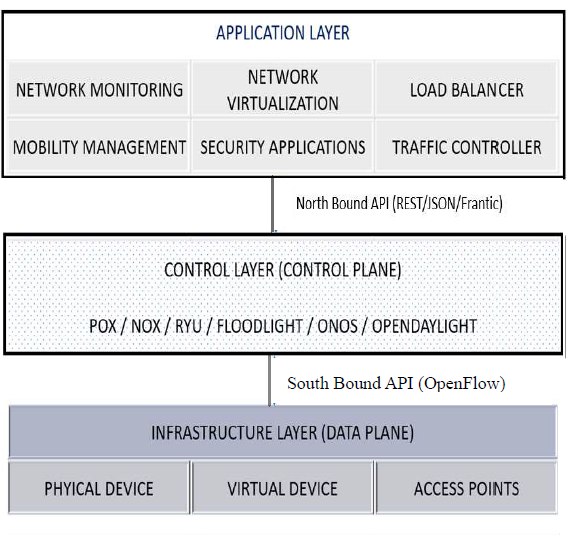
\includegraphics[width=10cm,keepaspectratio]{images/SDN-architecture-example.png}
    \caption{SDN Architecture \cite{sdnimages}}
    \label{fig:SDN Architecure}
\end{figure}
    
    As described above, the software-defined network follows a divide and conquer approach to networking \cite{taxonomy2014}. Instead of making each and every router in the network to perform both the tasks of finding an optimal route to the destination, storing it to its own 'routing table' for future reference and notifying its neighbors of the change and at the same time, forwarding data packets of other predefined routes, it is load has been reduced and made to solely focus on data forwarding, by looking at a 'flow table' rather than calculating a route and updating it. In case it needs a new route, or if any predefined routes get obsolete, it merely pings the controller and complies.
    
     The controller performs all the functions of calculating routes, monitoring network topology, and checking network health. This provides a centralized interface to manage the entire network. The benefit of such a system is that there is no need to communicate the status of the network to the entire network. Instead, simply dump all information onto a central device or a collectively operating set of devices, and it will make sure that the network runs smoothly and in the most hassle-free manner.
     
    Another advantage of using a separate entity for controlling the network is that it allows the network to be protocol independent. In other words, the operating system or the software that is running on the controller is not fixed. The software-defined network architecture allows us to change the operating system whenever required \cite{arpanet2004}. Granted, it will be a time-consuming task before the network is up and running again, but it certainly is a quicker and cheaper alternative to having to change the software on all the devices in the network.

    In any technology, the rewards will always come at either a trade-off or at risk. From slow but convenient transportation of the bicycle to the spectacular but risky aviation technologies, development always comes at a cost.
    Similarly, in software-defined networking as well, there are some bills to be paid.
    
    Firstly the implementation of a collective entity called the controller is in the way of putting all eggs in one basket. This method, however efficient, still poses a risk. The general principle in any management technology is to increase redundancy. If, for a sizeable software-defined network, there is a single controller, in case of any faults ranging from power outages to natural disasters can cause the entire network to fail.  
    
    Another downside of software-defined networking is that the central controller does not necessarily monitor the actual traffic itself rather only the network's health and different routes. It does not necessarily monitor the traffic is because controllers are capable of monitoring network traffic using third-party applications. It is physically possible for the controller to continuously ping a switch in order to get the packets it handles and read its contents. However, it is incredibly impractical, and therefore pursuing such a feature would yield fewer returns than the effort put in. So naturally, developers do not focus on traffic monitoring as much as compared to network monitoring and routing. This significantly reduces the scope of software-defined networking as networks in which traffic cannot be monitored efficiently would pose a risk in terms of authenticity and privacy. Unless the entire network is trusted by the network administrator and the network participants, such a method would seem less preferred.
    
    Last but not least, as an extension to the points prior to the previous one, since a single entity controls the entire network's routing and monitors the network health and topology, this will obviously result in a severe overhead on the controller. It was mentioned that software-defined networks are operating system independent, but they are, in a way, dependent on the hardware limitations. Such as processing power, network bandwidth, and will prevent the network from growing beyond an absolute scale. As the network scales, so does the complexity in handling such an extensive network. Tasks such as routing, topology discovery \cite{netflow2004} become cumbersome unless the controller hardware is upgraded.
    
    Also, this makes the network elastic, meaning it tends to want to return to its original dimensions, due to overstress on the controller. Unless the controller device is changed, which, although not that expensive or time-consuming, generates a degree of unreliability in the network, in traditional networks, load balancing on routes would be performed by neighboring routers, and the task of network monitoring was delegated, this meant that the network overhead would never go beyond a limit. In case all the routers in the network reached its limit, merely adding more routers and breaking down large networks to smaller subnets would be enough. However, that is uncertain in the case of software-defined networks. Distributed controllers solve this problem to an extent, but still need more time to develop into a more robust approach.
    
    \section{Motivation \& Problem Statement}
    
    Software-Defined Networks brings a new perspective to network architectures. The concept of having a centralized approach to decentralized network architecture brings the merits of both architectures. SDN architecture provides the infrastructural flexibility and robustness of the traditional networks with the added feature of having a central interface to monitor and manage the entire network.
    
    There are many SDN implementations, each with a different controller operating system. However, there comes a question to choose the suitable controller for a network scenario where there are limited resources. Here, controllers are analyzed and tested for system-level performance metrics under a massive network traffic that appears similar to real-world networks. It helps to identify system-level bottlenecks of the controllers and makes it possible to classify controllers based on their system performances. It also generates the idea of whether the provided system is suited to a given controller and vice-versa.
    \chapter{Literature Survey}

A starter handle of SDN was required to get hypotheses and details that assume significant jobs in the system. The paper underneath was critical for looking for data on the changed networking frameworks that were being used and how a product characterized arrange was distinctive in contrast with the traditional network design.

Published in 2014, the paper ``A survey and a layered taxonomy of software-defined networking'' \cite{taxonomy2014} puts forward a system that classifies published research works and brings to light the proper path to pursue research. The paper described that there is a need to classify and compare SDN Controllers but from a different perspective. Rather than just measuring raw performance, the scenario must be considered in which the operating system ,runs as well as what the network's objective is.

Also, the paper titled `` Software-defined Networking (SDN): a survey ''\cite{benzekki2016survey} and published in 2016, apart from the description about SDN, its controllers and architecture, it provides details about the issues prevailing in adopting SDN by existing networking giants.

Further research was done to understand how to compare different network operating systems. There are many open-source network controllers available. But in order to find the best controller, first, there is a need to establish the meaning of "the best controller" or whether there is any relevance to such a concept.

A paper published in 2014, titled ``Software-Defined Networking: A Comprehensive Survey'' \cite{Survey2014} performed an analysis of the hardware infrastructure used in the software-defined network architecture. The network uses simple switch like devices in place of fully functional routers. While data forwarding elements became dumb, the overall efficiency of network traffic significantly improved as routers were effectively simple programmable packet forwarding devices. The control plane elements are now represented by a single entity called the "Controller" or network operating system. Further third party applications are also allowed to be implemented on top of the network logic with authorization from the controller in order to provide some features specific to the operating system and are much easier to develop and deploy.

In order to compare controllers, first, there is a need for a set of metrics and tools with which the controller's performance can be identified and further classified based on network scenarios.

Published in 2016, the paper ``SDN Controllers: A Comparative Study'' \cite{adaptiveroute2006}  used CBench to test the performance of different controllers. The authors compared controllers based on factors that would yield an overall best performing controller. Their results concluded that controllers coded by the C language gave the highest performance in general along with Java-based distributed controller OpenDaylight.

Published in 2015, the paper ``On the performance of SDN controllers: A reality check'' \cite{realitycheck}  also used CBench to test the throughput and latency of 5 different controllers (Pox, Nox, Ryu, Floodlight, and Beacon). Their results concluded that Beacon has a better performance. Also, they concluded that Ryu is easy to learn and highly accessible.

Published in 2018, the paper ``Performance Analysis of POX and Ryu with Different SDN Topologies’’ shows a comparative study between two python-based controllers and tests them under different network topologies. It concludes that Ryu outperforms Pox in terms of throughput and latency.

Now the measurements that were generally used to look at SDN controllers were comprehended, there is a need to discover appropriate instruments and experiments. The following paper provides information as a part of collecting a choice of tools for our experiment.

Published in 2014, the paper ``Using Mininet for Emulation and Prototyping Software Defined Networks'' \cite{mininet2014} is on the study of SDN controller emulation techniques and tools such as Mininet. Mininet creates a realistic virtual network, running real kernel, switch, and application code, on a single machine (VM, cloud, or native), in seconds, with a single command.

Published in 2018, the paper ``Benchmarking Methodology for Software-Defined Networking (SDN) Controller Performance'' \cite{rfc8456} defines a set of metrics and corresponding methodologies for benchmarking the control-plane performance of Software-Defined Networking (SDN) Controllers.

Published in 2019, the paper titled ``SDN Controllers: Benchmarking \& Performance Evaluation'' \cite{zhu2019sdn} not only show results on comparative performances of various SDN Controllers but also provide a comparative study on various tools like CBench. It also includes the CPU Utilization Analysis, where OFNet is used to send bulk packets.

Published in 2012, the paper ``A Flexible Open-Flow Controller Benchmark’’ \cite{flexible} proposes changes to the OpenFlow protocol as they discovered inherent CPU performance bottlenecks. It also shows how multiple instances of CBench is used to send packets and measure CPU utilization.

Published in 2014, the paper titled ``OFCProbe: A platform-independent tool for OpenFlow controller analysis’’ \cite{ofcprobe} shows both OFCProbe and OFCBench being used as a CPU and RAM utilization monitor and finding bottlenecks for the controller. However, both only works with Ryu, Floodlight, and Nox. It implements the CPU and RAM monitors at the host machine using SMTP messages.

\section*{Summary}

The literature survey involved publications related to either explanation of fundamentals and concepts of software-defined networking, or research indicating different applications of controllers in software-defined networking based on real-world scenarios. Some papers also discussed methods of comparing controllers based on performance and other relevant factors. Different metrics used for controller performance comparison were used, and the relevance of those metrics was also discussed. The survey clarifies that there is a need for a comparison of different controllers. Previous papers mostly published performance results of controllers based on network size, throughput, and latency. Those who published about system utilization only include information about CPU and RAM and excluded information about cache memory, etc. which are also major factors in performance. Furthermore, the tools necessary for sending bulk packets to the controller operating system, such as OFNet, is now a dead project and is not available. OFCBench and OFCProbe use SMTP messages to get data from the controller and are limited to a few Benchmarks, whose data is less accurate.
    \chapter{System Utilization of SDN/OpenFlow Controllers: Ryu Versus Pox}

    There are different SDN controllers available. Some of them are open source projects developed and maintained by the community, while private organizations develop some. Regardless of open source or private, all controllers follow the same principle of hardware independence and the divide and conquer approach. As with any case where there are multiple options of one thing, a choice is made because we cannot deploy all the options in the same environment simultaneously.
 
    To select the best controller, first, there is a need to understand the concept of the best controller. What are the criteria on which controllers need to be judged or compared? Is there even a possible best controller among them all. Similar to how we measure distance using a ruler, or time using a clock, we need a standard against which controllers can be compared, and then compare the comparisons with each other. This standard of metrics is crucial to selecting which controller would be ideal. There are some papers which mention a few relevant metrics, let us take a look.
    
    Controllers must be compared on several criteria. Previous papers discussed a wide variety of properties of controllers ranging from physical performance to fault tolerance. Some of the metrics include time for setting up the network, tearing down the network, processing power Usage, Potential to scale the network, CPU utilization, memory usage, throughput, latency, ping delay, no Response failure rate, a fair share of resources.
    
    These metrics give a fair idea of the performance of the controller on an industrial level. Nevertheless, all these criteria seem well researched and are continually evolving with upgraded hardware and new features in the software. Factors like system utilization also have to be evaluated to determine whether the controller uses the hardware constraints efficiently. It also gives a clear idea about the controller's nature while it is running and helps identify the system bottlenecks.
    
    A paper published in 2018 came up with methodologies for measuring the performance of all controller implementations and benchmarked the control- plane performance \cite{rfc8456}.
    
    Another paper, published in 2019, describes a repetitive series of tests using a network emulator and a benchmark tool that included the CPU utilization of various Controllers on a machine. It uses a benchmark tool which operates on a different system, that sends a considerable amount of random packets to the controller and then reads CPU utilization values. Fig. \ref{figzhu2019sdn} below depicts the average CPU utilization at a given time. The graph gets populated by data from the benchmark tool, which performs the test seamlessly. At the same time, the controller operating system runs on a virtual machine \cite{zhu2019sdn}. Currently, the benchmark OFNet used in that experiment is no longer available as the concerned owner has removed it.
    
    A paper, published in 2014, describes how OFCBench and OFCProbe can be used as CPU and RAM utilization monitor and find bottlenecks of the controller. The implementation of these monitors is by sending SMTP messages from client machines. However, it is worth noting that both these tools are limited to work with Floodlight, Ryu, and Nox Controllers. \cite{ofcprobe}
    
    One more paper, published in 2012, shows they used multiple instances of CBench to send packets and measure the CPU Utilization. They discovered an inherent performance bottleneck concerning CPU load in OpenFlow switch implementations of those days. \cite{flexible}
    
\begin{figure}[!hbt]
    \centering
        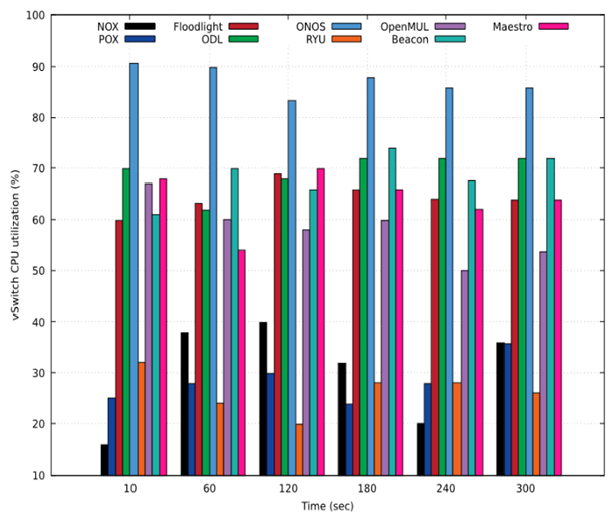
\includegraphics[width=\textwidth,keepaspectratio]{images/zhucpu.png}
       \caption{CPU Utilization Results Published \cite{zhu2019sdn}}
        \label{figzhu2019sdn}
\end{figure}

    The throughput mode of CBench in which the switches are configured to wait and pile up a set of requests and send all the requests at once to the controller. This forces the controller to allocate a significant share of its resources to one or two switches at a time. This technique measures the stress capacity of the controller. The controller must have enough memory to store and process all the requests from a switch. It need not be able to run so many threads at the same time.

    The tests performed in the paper \cite{dynamicrouting} consider many controllers, running in a network whose size increases. For this feature, they increased the number of nodes after each set of tests and repeated them while recording the results. The thing that seems overlooked in this test is that the results are valid, provide us only with a basic idea of the controller's performance. The controller with the best growth of response rate in proportion to network size was classified as the best controller.
        
    The controller provides more responses as the network size increase. It is because there is more packet in events from switches. As the network size increases, more routes need to be calculated and maintained. More switches need to be updated regularly. However, one factor is overlooked. The fact that more requests are generated is not necessarily because there are more switches; it is because there are more hosts overall connected to the network. The experiment performed as in paper \cite{routingtie2017} by increasing the number of switches while maintaining the number of hosts per switch. As the network grew, more hosts would want to communicate, thus leading to the rise in route requests or packet in events.
    
    \textit{Traffic Intensity} is a measure of how flooded a network is with traffic. As the network gets scaled up, the number of hosts increases, thus increasing traffic Intensity. This increase in traffic intensity forces the controller to increase its performance rates to cope with the network requirements. There is a need for a method to compare controller such that minimum external factors are influencing the controller's performance. Here, the traffic Intensity is kept quite high, changing the network topology to see how different controllers handle the scenario and how their performance is affected.

    For any test, the environment within which the subject to be tested must be isolated from external factors as much as possible. In the case of testing and performing a benchmark on SDN controllers, the cores of CPU where the controller runs, needs to be isolated using \textit{isolcpus} or similar tool.
    \chapter{Experimental Setup}
Two open-source controllers operating systems were compared. Ryu and Pox are installed on a server machine. Conversely, Mininet and CBench are introduced on two distinctive host machines in the accompanying equipment and programming arrangements.

 \begin{table}[!hbt]
    \centering
    \caption{Features of Pox and Ryu \cite{ryuandpox}}
    \begin{tabular}{|p{4cm}|p{4cm}|p{4cm}|}
    \hline
         \textbf{Features} & \textbf{Pox} & \textbf{Ryu} \\ \hline
         Platform Support & Windows, Linux, Mac & Linux \\ \hline
    Last Updated & Nov 2017 & May 2020 \\ \hline
    License Provider & Apache & Apache \\ \hline
    Distributed Support & No & Yes \\ \hline
         Learning Curve & Easy & Moderate \\ \hline
         GUI & Yes & Yes \\ \hline
    REST API & Yes & Yes \\ \hline
    OpenFlow Version & v1.0 & v1.0 to v1.5, Niciria extensions \\ \hline
    \end{tabular}
    \label{RyuvsPox}
    \end{table}
    
\section{Hardware Configuration}
    \begin{table}[!hbt]
    \centering
    \caption{Physical constraints of Server and Host Machines}
    \begin{tabular}{|c|c|}
    \hline
    Architecture & x86\_64 \\ \hline
         CPU op-mode(s) & 32-bit, 64-bit \\ \hline
         CPU(s) & 8 \\ \hline
         Thread(s) per core & 2 \\ \hline
         Vendor ID & GenuineIntel \\ \hline
    Model name & Intel(R) Core(TM) i7-4790K CPU @ 4.00GHz \\ \hline
    L1d cache & 128 KiB \\ \hline
    L1i cache & 128 KiB \\ \hline
    L2 cache & 1 MiB \\ \hline
    L3 cache & 8 MiB \\ \hline
    \end{tabular}
    \label{Hardware}
    \end{table}

The setups, as referenced above, were not deliberately picked; rather, it was the asset limitations during the task's time. All things considered, these designs could be additionally changed dependent on rehashed tests. Thus, even the most exceedingly terrible performing controller is best considering the constrained preparing force and RAM.

\section{Software \& Tools}
The controller is run on a Linux Ubuntu Server 18.04 LTS OS so that it got dedicated RAM and processor cores \cite{resshare1970}, and 5 out of 8 cores were isolated for the controller using \textit{isolcpus} tool.

Perf was also installed along with the controllers on the server machine itself but on a different single isolated core to prevent influence from any other running process(s).

Oracle VM VirtualBox is installed on two separate host machines. An instance of Linux Ubuntu Desktop 16.04.02 LTS OS is created.

Mininet is installed on the Host OS and is used to set the hosts, switches, controllers, and set any possible combinations of connections.

CBench device copies a lot of switches and hosts per switch and interfaces with the SDN controller indicated. Generally, it creates them in the network and measures the presentation of the controller in 2 modes.
    \begin{itemize}
        \item Latency Mode: Packets in these events come in bulk from each switch.
        \item Throughput Mode: Packets in events come in sequential order.
    \end{itemize}

\begin{figure}[!hbt]
    \centering
        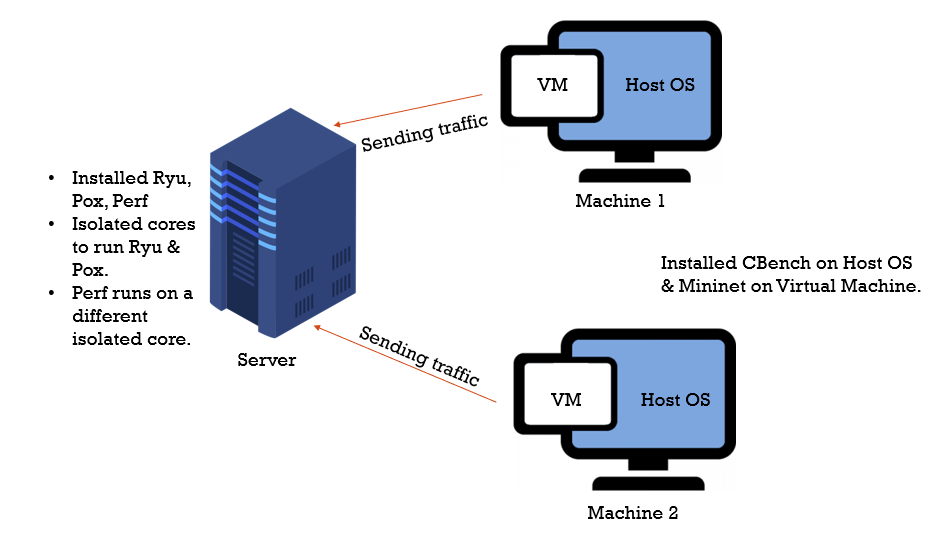
\includegraphics[width=\textwidth,keepaspectratio]{images/setup.png}
       \caption{Experimental Setup}
        \label{experimentalsetup}
\end{figure}

\begin{figure}[!hbt]
    \centering
        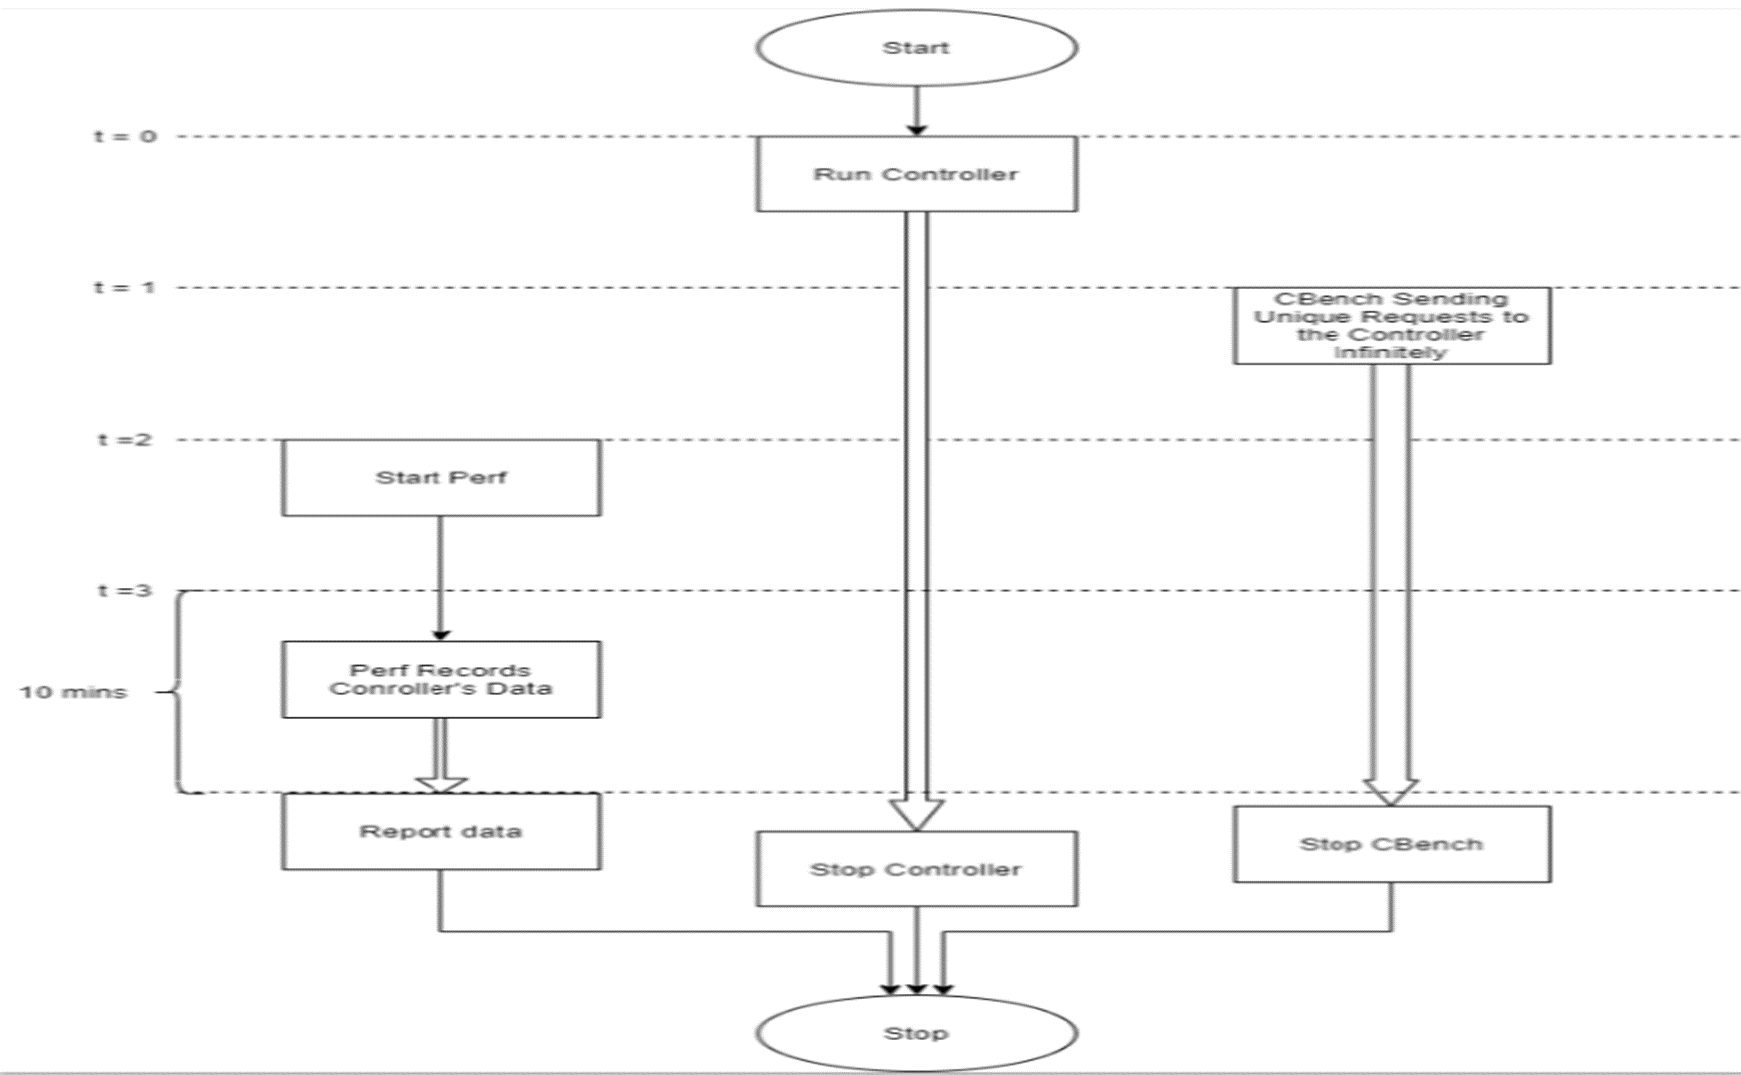
\includegraphics[width=\textwidth,keepaspectratio]{images/Workflow.PNG}
       \caption{Workflow of the Experiment}
        \label{workflowexperiment}
\end{figure}

However, in our case, we took the usage of CBench in throughput mode and generated massive traffic for the controller.

The overall experimental setup can be viewed as in Fig. \ref{experimentalsetup}. The Ryu and Pox along with perf, are installed on server machine, and whenever they are run, were run on isolated cores. In the experiment, 6 isolated cores are assigned for Pox. In one of the isolated core, perf is allowed to run. In the experiment, there are 2 hosts / client machines used. These two machines was set to send traffic to the server where controller is running. In both of the hosts, CBench is installed, and further Mininet is installed on a separate virtual machine in the system.

The experiment is carried on as the per the workflow, depicted in the Fig. \ref{workflowexperiment}. The controller is allowed run on isolated cores. Then the CBench and Mininet is allowed to send random packets to the running controller from other two remote machines. Perf tool is run to record the cores where controller is running for specified time and later stopped. This is done for both Ryu and Pox, and a number of times (here 5 times) to get relatively more accurate information. The information collected is further displayed in graphical chart using Google Chart.
    \chapter{Results \& Discussions}

All the published papers declared results for their experiment where the controllers were tested either for CPU or RAM utilization. They performed tests using the OFNet tool to create a vast virtual network, send large packets to the server, and use OFCProbe or OFCBench to monitor the CPU and RAM utilization via the use of SMTP messages. However, instead of OFNet, multiple instances of CBench can also be used to send those packets.

In our experiment, we have used multiple instances of CBench and Mininet. We have also used Perf to read the system utilization information directly at the server.

After having our experiment, as illustrated in the workflow depicted in Fig. \ref{workflowexperiment}, the collected raw data is represented in a graphical format. We received and processed the system metrics such as CPU Utilization, Clock Speed, Instructions per Second, Branch mispredictions, and various level cache miss rates. These results are further discussed one by one.

\section{CPU Utilization}

\begin{figure}[!hbt]
    \centering
        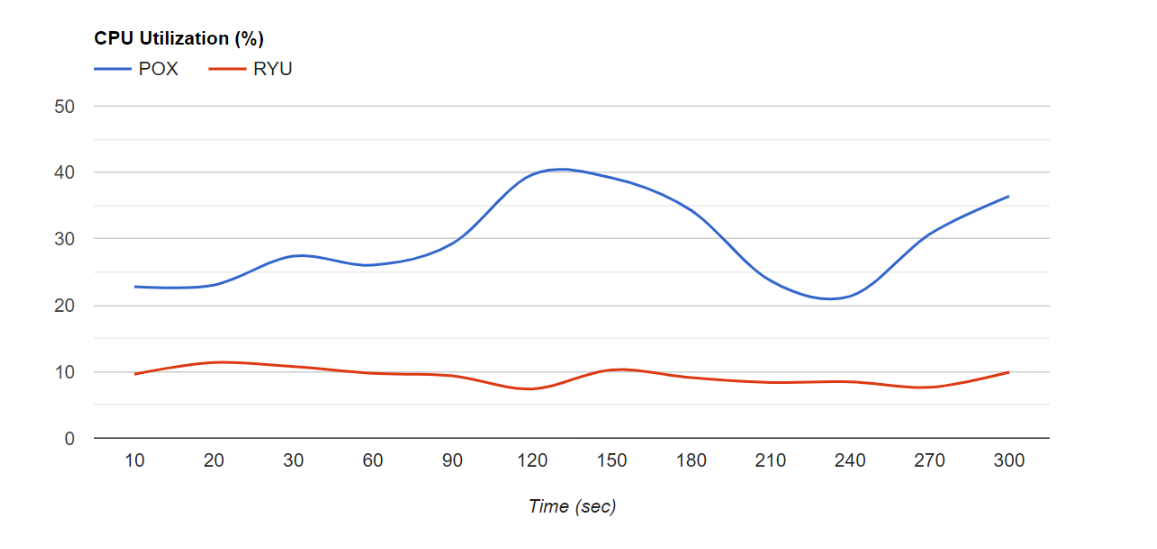
\includegraphics[width=\textwidth,keepaspectratio]{images/cpu_utilization.png}
       \caption{CPU Utilization}
        \label{CPUutilization}
\end{figure}

Usage of the CPU refers to the use of computing power by a process or the amount of work a CPU performs. Specific tasks require massive CPU time, while others require less because of non-CPU resource requirements. A method is said to be working better if, for the same number of tasks, it utilizes less CPU.

In our result, it shows that RYU continuously utilizes less CPU than POX, depicted in Fig. \ref{CPUutilization} However, it was not such as seen in Fig. \ref{figzhu2019sdn} taken from the paper published in 2018, that depicted for at least fewer time Pox too utilize the same as Ryu or even less CPU. \cite{zhu2019sdn}

\section{Instructions Per Second}

Instructions per Cycle (IPC), generally referred to as clock instructions, are one component of processor performance: the total number of instructions per clock cycle.

\begin{figure}[!hbt]
    \centering
        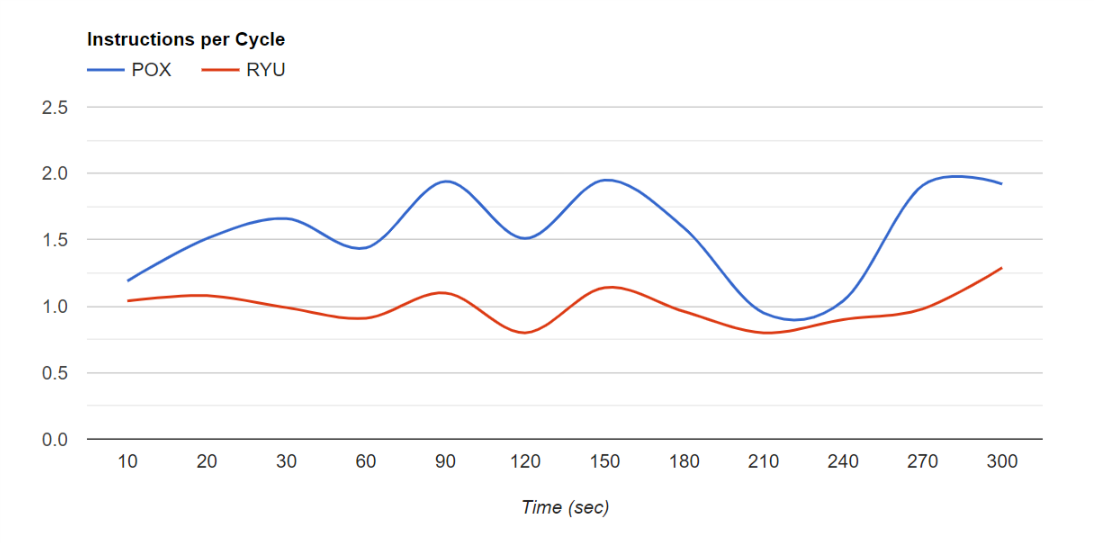
\includegraphics[width=\textwidth,keepaspectratio]{images/ipc.png}
       \caption{IPC}
        \label{ipc}
\end{figure}

With a specific processor, the number of instructions executed per clock is not a constant; it depends on how the individual program running communicates with the processor, and indeed the entire system, particularly the memory hierarchy. Nonetheless, certain CPU characteristics tend to contribute to designs with higher than average IPC values; the inclusion of several arithmetic logic units (an ALU is a CPU module capable of performing basic arithmetic and logical operations); and short pipelines. When evaluating various instruction sets, a simplified instruction set will contribute to a higher IPC number than applying a more complicated instruction set with the same chip technology; furthermore, with fewer instructions, the more complex instruction set may do more valuable work. 

The obtained result is depicted in Fig. \ref{ipc}. The efficient use of pipelining can be seen by both the controllers where both scored IPC values greater than 1. However, Pox, in contrast to Ryu, has better IPC.

\section{CPU Clock Speed}

CPU clock speed is calculated in Hertz — generally in gigahertz or GHz. Clock speed is a function of how many
clock cycles a Processor will execute per second. For example, a 1.8 GHz clock-rate CPU will execute 1,800,000,000 clock cycles per second. It looks so plain on the face. The more cycles a CPU can perform, the more it can do.

\begin{figure}[!hbt]
    \centering
        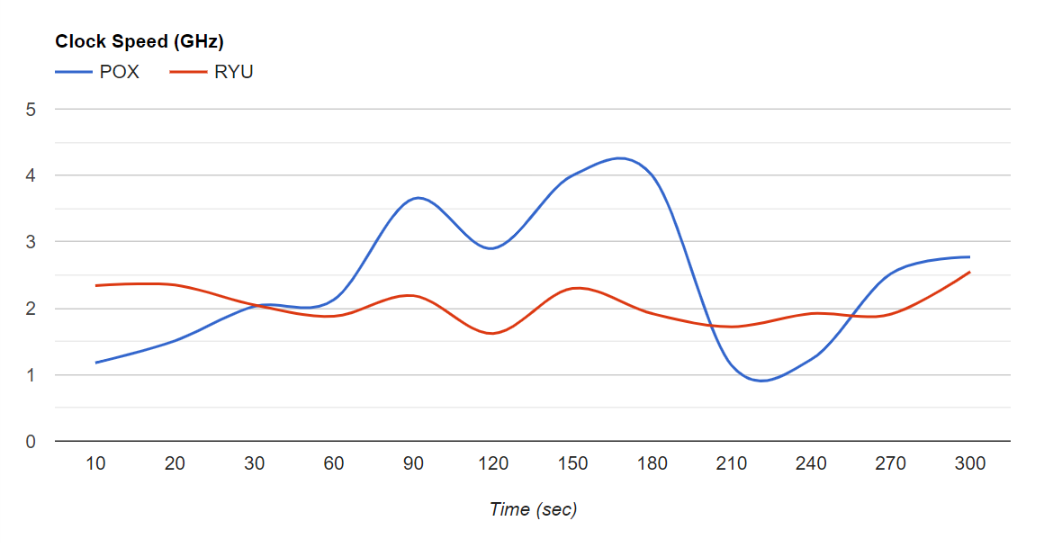
\includegraphics[width=\textwidth,keepaspectratio]{images/clock_speed.png}
       \caption{CPU Clock Speed}
        \label{clockspeed}
\end{figure}

On average both Ryu and Pox relatively has a similar clock speed of about a 2GHz. However, it is also seen from Fig. \ref{clockspeed} that Pox even touches a 4GHz score or more when required. Thus, confirming that the controller uses the Turbo Boost features provided by the system used for the experiment.

\section{L1 Cache Miss Rate}

In order to improve the performance of the cache, reducing the missing rate becomes one of the necessary steps. Decreasing access time to the cache also boosts its performance.

\begin{figure}[!hbt]
    \centering
        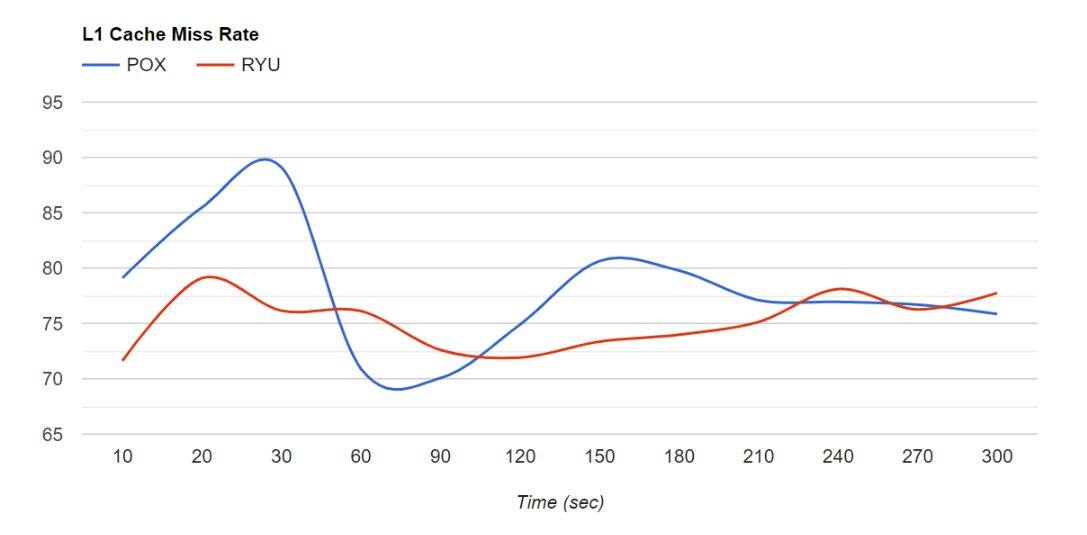
\includegraphics[width=\textwidth,keepaspectratio]{images/l1_miss_rate.png}
       \caption{L1 cache miss rate}
        \label{l1missrate}
\end{figure}

From the experiment as depicted in Fig. \ref{l1missrate}, it can be observed that on average, both Pox and Ryu has 80\% and 75\% of l1 miss rates respectively. This high miss rate is not enough for any real-time applications. However, during the initiation phase Pox even has the miss rate as high as 90\%.

\section{L2 Cache Miss Rate}

\begin{figure}[!hbt]
    \centering
        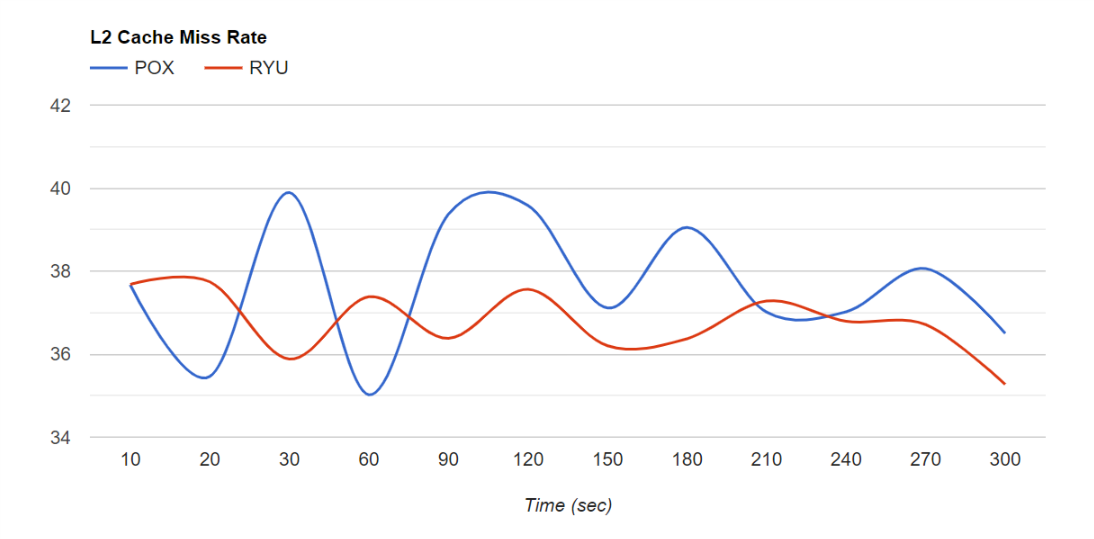
\includegraphics[width=\textwidth,keepaspectratio]{images/l2_miss_rate.png}
       \caption{L2 cache miss rate}
        \label{l2missrate}
\end{figure}

For level-2 cache, the miss rates are quite less than as compared to level-1 cache. The L2 miss rates for Ryu and Pox is observed to be below 40\%. However, about real-time applications that need to run 24*7 less than the observed.

\section{Branch Misprediction}

Branch Predictions are an architectural innovation that provides an alternative to conditional control transfers, enforced by computer commands, such as conditional branch, conditional call, tentative return and tables for branches. Predication operates by implementing instructions from both branch directions, enabling only specific instructions from the path taken to change architectural condition.

\begin{figure}[!hbt]
    \centering
        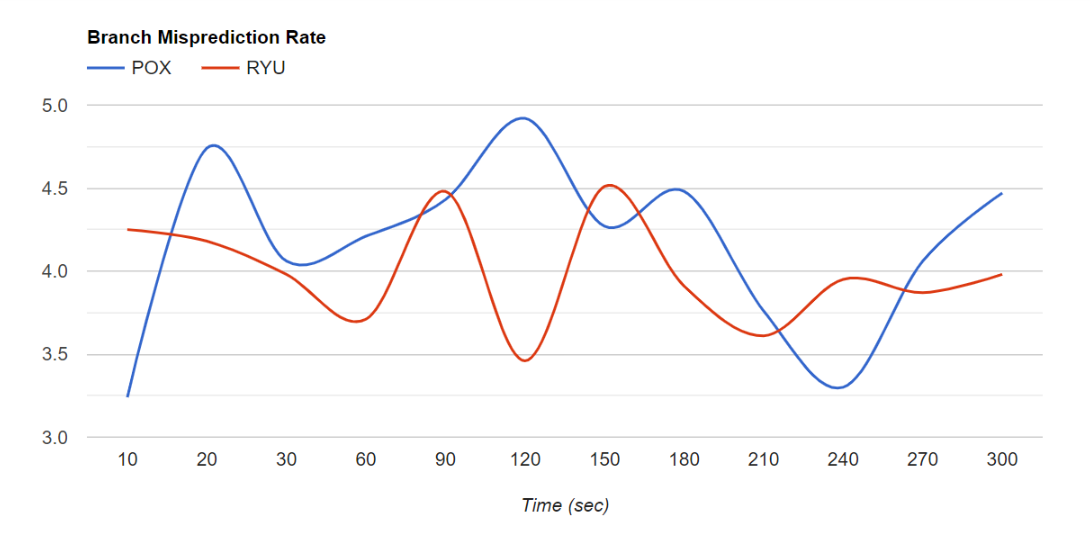
\includegraphics[width=\textwidth,keepaspectratio]{images/branch_mispredicted.png}
       \caption{Branch Misprediction Rate}
        \label{branchmisprediction}
\end{figure}

The branch predictor aims to boost flow inside the instruction pipeline. In several modern pipelined microprocessor architectures such as x86, branch predictors play a critical role in achieving highly effective performance. Predictor latency can also have
a profound impact on efficiency. Branch Misprediction Rate is the ratio that indicates the rate of mispredicted branches.

When there is a high rate of a branch misprediction, an optimization (minimization) problem is used where the
emphasis is on achieving the lowest possible miss rate, low power consumption and low resource complexity. 

As shown in Fig. \ref{branchmisprediction}, the result clearly shows, for both Ryu and Pox, this rate is quite low, i.e. below 5\%. Also, during initialization time (first 10 - 15 secs), Pox has this rate significantly lesser than Ryu. However, overall on average, Ryu has about 22\% fewer misprediction rates than Pox.
    \chapter{Conclusion \& Future Works} 

The experiment was successfully performed on two different SDN controllers (Ryu and Pox) as planned under heavy traffic and with the latest stable releases of both controllers. The results provide a clear picture of their system-level performances. It also shows system performance analysis of SDN controllers is a challenging task.  It can be observed that Ryu utilized less CPU than Pox as the former does not support multi-threading while the later does. The utilization of first level cache by both the controllers was reduced and scored more than 70\%. However notably, both controllers efficiently use other higher-level caches and branch predictors. Further is also observed that both controllers have a decent score of instructions per cycle, i.e. greater than 1, which signifies the pipelining is used efficiently. Pox even has a better efficiently coded initializing module(s) than of Ryu's, as seen from the lesser branch mispredictions and higher IPC during the starting time.

This experiment also makes itself different and competitive from others as it was performed under heavy traffic and analyzed on the latest releases of both controllers. Since OFNet is no longer available \cite{}, this experiment successfully shows the efficient mutual use of CBench and Mininet to send random packets.

The use of the perf tool in the experiment shows how this tool is capable of measuring system-level metrics right from the server itself, rather than using OFCBench or OFCProbe which were limited to Floodlight, Ryu and Nox and also ran on host machines, sending SMTP messages to get data from server.

In future works, some of the limitations faced by this research could be looked into, such as the lack of hardware and time. This experiment also displayed how system bottlenecks identification can be made, which will help the developers to improve SDN Controllers running on a server and also identify which system will be better for a given controller or which controller will be better for a given system. This experiment also lays down information to help developers know about the programming lags. It thus will help them write more optimized modules of SDN Controllers to utilize the system better. This type of profiling will also encourage to use the compilers like LLVM, Numba, etc. to develop or improve controllers.

Unlike OMNET++, a popular network application used to simulate computer networks has been a part of SPEC CPU Benchmark Suite since 2006; one of the various SDN Controllers also have a higher possibility, viewing the increasing popularity among multiple networks and hardware corporate giants, that controller will be developed using the profiling as done in this experiment.
    \addcontentsline{toc}{chapter}{Bibliography}
\printbibliography
    \chapter*{Annexure - A}
\addcontentsline{toc}{chapter}{Annexure-A}

\section*{Tools used for Creating Virtual Environment}

\begin{itemize}

    \item Ubuntu Server 18.04 LTS \\
    $https://releases.ubuntu.com/18.04.4/ubuntu-18.04.4-live-server-amd64.iso$
    \item Oracle VM Virtual Box \\
    $https://download.virtualbox.org/virtualbox/6.1.8/$
    
\end{itemize}

\section*{Tools used for Emulation of Controllers}

\begin{itemize}

    \item Mininet \& OpenVSwitch \\
    $http://mininet.org/download$
    \item Ryu \\
    $git\ clone\ https://github.com/faucetsdn/ryu.git$
    \item Pox \\
    $git\ clone\ https://github.com/noxrepo/pox.git$
    \item CBench \\ 
    $git\ clone\ git://gitosis.stanford.edu/oflops.git$
    
\end{itemize}

\section*{Tools used for System Monitoring}

\begin{itemize}

    \item Perf \\
    $apt\ install\ linux-tools-\$(uname -r) linux-tools-generic$
    \item htop \\
    $sudo\ yum\ install\ htop$
    
\end{itemize}
    \chapter*{Annexure - B}
\addcontentsline{toc}{chapter}{Annexure-B}

\section*{Implementation of OpenVSwitch}

\begin{itemize}

    \item Mininet Configuration
        
    \begin{itemize}
    
        \item Command from mininet installation folder\\
        \emph{sudo python miniedit.py}
        
        \item Select controller type as OpenVSwitch and press Run. The controller will listen for switches to port 6633 on localhost ip address
            
    \end{itemize}
    
    \item Cbench Configuration
        
    \begin{itemize}
    
        \item Command from Cbench installation folder\\
        \emph{./cbench -c localhost -p 6633 -s 16 -M 1 -t}\\
        to run the Cbench tool against 16 swtiches (-s) with 1 host (-M) per switch in throughput mode (-t) or latency mode (-l)
        at localhost controller ip (-c) on port 6633 (-p) 
        
        
    \end{itemize}
    
\end{itemize}

\section*{Implementation of OpenDayLight}

\begin{itemize}
    
    \item Vagrant Machine
    
    \begin{itemize}
    
        \item Command to boot up vagrant machine from installation folder \\
        \emph{vagrant up}
        \item Command to ssh into the vagrant machine\\\emph{vagrant ssh}
        \item Command to exit from Vagrant ssh \\ \emph{exit}
        \item Command to gracefully shutdown Vagrant machine \\ \emph{vagrant halt} 
        
    \end{itemize}
    
    \item WCbench Configuration within Vagrant
    
    \begin{itemize}
    
        \item Command to start OpenDayLight controller from location "/wcbench"\\ \emph{./wcbench -o}
        
        \item Command from location "/wcbench/cbench" to benchmark the controller\\
        \emph{./cbench -c localhost -s 16 -M 1 -t}\\
        
        to run the Cbench tool against 16 swtiches (-s) with 1 host (-M) per switch in throughput mode (-t) or latency mode (-l)
        at localhost controller IP address (-c)
        
        \item Command to stop OpenDayLight from location "/wcbench" \\ 
        \emph{./wcbench -k}
        
    \end{itemize}
    
\end{itemize}

\section*{Implementation of Floodlight}

\begin{itemize}
    
    \item Floodlight Machine 
    
    \begin{itemize}
    
        \item Open Virtual Box
        \item Load and Boot Up Floodlight Image
        \item Command to start floodlight controller within location "/floodlight"\\
        \emph{java -jar target/floodlight.jar}
        \item open separate terminal and run ifconfig to note down IP Address
        
    \end{itemize}
    
    \item Cbench Configuration
    
    \begin{itemize}
    
        \item Command from location "/wcbench/cbench" to benchmark the controller\\
        \emph{./cbench -c (IP Adress of floodlight controller) -p 6653 -s 16 -M 1 -t}\\
        
        to run the Cbench tool against 16 swtiches (-s) with 1 host (-M) per switch in throughput mode (-t) or latency mode (-l)
        at localhost controller IP address (-c)  on port 6653  
    
        \end{itemize}
    
\end{itemize}
    
\end{document}
